% !TEX root = ../control.tex

\section{引言}

角度测量在现代科学研究与工程应用中具有不可或缺的重要地位，广泛服务于精密制造、光学校准、航空航天系统定位与姿态控制、机器人视觉系统调试以及计量标准的建立与维护等诸多领域。高精度角度信息的获取往往直接关系到系统运行的可靠性与最终产品的性能质量，因此开发一种具有高分辨率、高稳定性且适用于复杂环境的角度测量装置，一直是精密测量技术的重要研究方向。

本报告聚焦于一种基于自准直原理，并辅以高分辨率旋转增量式光学编码器的角度测量装置的设计方案。自准直技术因其在微小角度变化测量方面展现出的卓越灵敏度和良好稳定性，已被广泛应用于对准检测、旋转轴误差分析、角度偏差测定等高要求测量任务中。其基本原理在于利用准直光束与被测面之间的反射偏差来表征角度变化，从而实现非接触、远距离的高精度测量。特别是在小角度测量场景中，自准直技术具有可观的优势。

然而，传统自准直器依赖人工读数或模拟图像分析，易受主观判断和环境因素干扰，且难以满足现代高集成化、高自动化测量系统的需求。为此，本文提出将自准直测量系统与高分辨率旋转光学编码器相结合，利用后者在数字信号处理方面的能力，实现对角度变化的精确量化与实时记录。这种复合式结构不仅保留了自准直测量的高灵敏度特点，同时通过光学编码器的引入有效提升了系统的可操作性与测量效率，具备优良的工程实用潜力。

本报告的后续内容将依次展开：首先明确装置的设计目标与核心性能指标，随后系统性阐述其工作原理，并结合原理图对关键物理机制进行建模与公式推导；接着详述整体结构设计与各主要组件的参数配置；随后开展初步的性能分析与误差分配，评估该方案在目标精度下的可行性；最后对该设计方案的优势、局限及适用范围进行总结讨论，以期为相关精密测量装置的设计与实现提供理论基础与技术参考。

\section{设计目标与指标参数}

\subsection{量程}

\YsyMark{本装置的设计测量范围设定为 ±5°，即相对于初始参考方向允许存在最大达 10° 的双向角度偏移。}

该量程设置旨在兼顾装置的高精度测量能力与广泛适用性，适合于涵盖绝大多数常见的角度测量应用场景。具体而言，±5° 的量程足以满足如机械结构装配对准、精密平台旋转误差评估、光学组件调整与校准等典型任务的需求。

在选定此量程的过程中充分考虑了测量任务对角度变化幅度的实际需求以及系统灵敏度与分辨能力之间的权衡关系。对于中等角度范围内的变化，传统自准直仪虽具备良好的灵敏度，但其测量精度易受光斑偏移非线性、反射面偏移超出视场等因素限制。因此，本装置在确保 ±5° 量程内维持高测量精度的前提下，通过精心设计的光学系统和高分辨率位置检测模块，使其兼具灵敏度与动态范围的协调统一。

该量程范围亦具备良好的扩展性。通过调整光路放大倍数或更换不同焦距的准直光学系统，装置亦可适配更大或更小范围的角度测量任务，从而具备一定的通用性与可重构能力。

\subsection{精度}

\YsyMark{本装置的目标角度测量精度设定为 1 角秒，对应弧度值约为 $4.85 \times 10^{-6}\text{rad}$。}

该精度等级对于多种对角度控制要求极高的应用具有关键意义，特别是在诸如高精度机械定位、精密旋转装置校准、干涉仪对准系统、天文望远镜安装调整等领域，其误差容限通常位于亚角秒级别，因而对测量装置提出了极高要求。

自准直技术因其测量角度偏差的方式为“反射式放大”，具备极高的角度灵敏度，是实现亚角秒级精度的理想选择。在经典自准直仪中，入射光束与被测面间形成的极小角度偏转将导致返回光束在像面上产生显著的线性位移，该位移可被高分辨率的探测元件（如 CCD、PSD）准确感知与量化。文献与现有高端商用设备表明，部分自准直仪可实现高达 0.1 角秒 的分辨能力，进一步验证了该测量原理在微小角度测量领域的可靠性与先进性。

因此，在合理的光路设计、噪声控制与误差补偿手段的支持下，基于自准直原理并结合高分辨率位置检测系统的测量装置，完全有可能实现 1 角秒以内的实际测量精度。该目标在技术上是现实可行的，同时也为本设计方案确立了明确的性能基准。

\subsection{分辨率}

\YsyMark{本角度测量装置的期望分辨率设定为 0.1 角秒，即约为 $4.85 \times 10^{-7}\text{rad}$。}

这一分辨能力使得系统能够分辨出极其微小的角度变化，对于精密机械定位、光学元件微调、纳米级对准系统等应用中的细节变化检测与反馈控制至关重要。

在精密测量系统中，分辨率代表系统对信号变化的最小感知能力，直接决定了测量系统对于动态或微幅变化的响应灵敏度。通常而言，为了确保测量数据的可靠性与有效性，仪器的分辨率应显著优于其目标精度，通常取精度的 5 到 10 倍。因而在目标精度为 1 角秒的设定下，配置 0.1 角秒分辨率的测量能力是合理且符合工程实践经验的。

自准直测量原理天然适合实现超高角度分辨率，其角度位移通过反射倍增转化为线性位移，使得角度变化可通过对光斑在成像面上的位移进行高分辨率检测予以准确反演。配合焦距较长的准直系统与高像素密度的探测器（如微米级精度的CCD或位置敏感探测器），理论上可实现甚至优于 0.1 角秒的位移感知。

尽管实现该级别的分辨率在系统稳定性、光学质量、电子噪声控制等方面存在一定挑战，但从原理上来看，依托自准直法的高放大因子与先进数字图像处理技术，该分辨率在技术上是可达的，亦为后续系统精度优化提供了坚实基础。

\subsection{为什么选择自准直法？}

在众多可用于角度测量的原理中，自准直法因其非接触性、高灵敏度与结构简洁性而成为本装置设计的首选方案。其核心优势在于：通过反射光路中微小角度变化所引起的光斑位移，可以实现对角度变化的高倍放大，从而在测量微小角度偏差时表现出卓越的分辨能力。

相较于干涉仪等结构复杂、对环境扰动高度敏感的方案，自准直法对环境要求更低，易于集成和稳定运行；相比光栅或磁栅编码器，其在小角度测量范围内具有更高的灵敏度和精度。此外，自准直技术在计量学领域已有长期成熟应用，理论模型完备，配套元器件齐全，工程实现难度可控，具有良好的可验证性和技术可靠性。

结合现代数字图像处理与高分辨率传感器的辅助，自准直法不仅能够实现高精度的角度测量，还能够通过数字化手段提升测量效率和抗干扰能力。因此，从测量性能、系统集成、工程可行性等多维度综合考虑，基于自准直原理的角度测量方案是实现本设计目标的优选路径。

\section{工作原理}

\subsection{光路与原理描述}

\begin{figure}[h!]
	\centering
	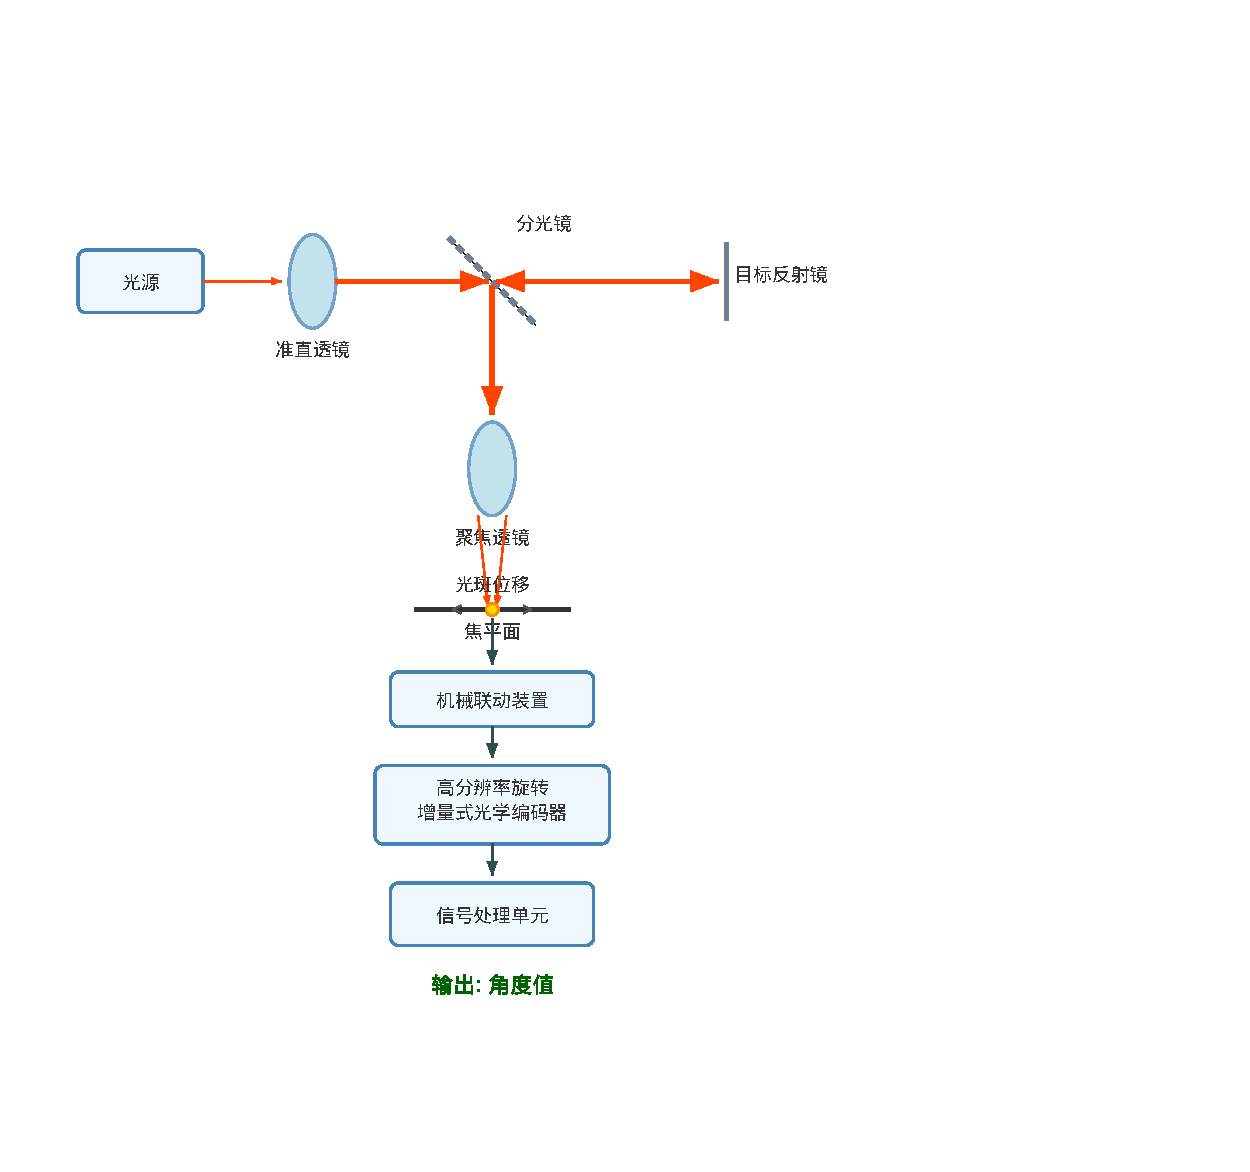
\includegraphics[width=0.7\linewidth]{images/ipm_hw_2_schematic}
	\caption{系统采用稳定的激光光源（如氦氖激光器）发出光束，经过准直透镜形成平行准直光。准直光经分光镜反射后射向被测目标反射镜。目标反射镜将光束沿原路径反射回自准直光路，反射光束再次通过分光镜并进入聚焦透镜，被聚焦至焦平面上。焦平面上的光斑位移通过机械联动装置转化为旋转运动，该旋转量由高分辨率旋转增量式光学编码器测量，信号处理单元对编码器输出进行解析，从而实现角度变化的高精度测量与数字化输出。}
	\label{fig:ipmhw2schematic}
\end{figure}

如\cref{fig:ipmhw2schematic}所示，本设计所提出的角度测量装置基于\YsyAnnotation{自准直原理}运行，整体光学路径与测量机制构建在经典反射几何与高灵敏度角度响应的基础之上。该原理的核心在于：通过监测光束在反射路径中的微小偏转，推算出目标反射面的角度变化，从而实现非接触式、高精度角度测量。

在系统工作过程中，稳定的激光光源（如氦氖激光器）发出高相干性且低发散角的激光束。该光束经由准直透镜转化为平行光，作为准直光束沿预设方向传播。该准直光随后通过一块分光镜偏折，引导光束垂直照射在待测物体上的高反射率平面镜（即目标反射镜）表面。

当目标反射镜的法线方向与自准直光轴完全重合时，光束沿原路返回，并经由分光镜的另一通道被引导至接收光学系统；若目标反射镜发生微小倾斜，则反射光束的传播方向将发生相应偏转。根据反射定律，镜面倾斜角 $\theta$ 会导致返回光束相对于入射光束发生 $2\theta$ 的角度偏移。这一倍增效应使得微小角度变化被有效放大，从而极大地提升了系统对微角度变化的响应灵敏度。

被偏转的光束在返回路径中进入聚焦透镜，被聚焦于像平面上形成光斑。反射镜角度变化导致光束偏转，其结果是在焦平面上产生可测的光斑横向位移。系统通过设计合理的光学焦距与探测面布局，使该位移与反射镜倾斜角呈线性近似关系。

为实现高精度数字化测量，本装置进一步引入\YsyAnnotation{机械联动放大机构}，该机构将焦平面上的微小光斑位移转化为机械旋转运动。旋转运动被传递至\YsyAnnotation{高分辨率旋转增量式光学编码器}，后者将角度变化以离散数字脉冲或编码信号输出。该编码信号具有固定分辨单元，可通过内部插值技术实现亚角秒级角度变化的采样与输出。

编码器输出由信号处理单元采集并实时解析，经由解码、滤波与校准等处理环节后，转换为可供分析与控制使用的数字角度数据。整个系统实现了从光学角度变化的感知、物理量的转换到最终数字化表达的完整测量链条，具备\YsyAnnotation{高灵敏度、高稳定性与高集成度}等显著特点。

综上所述，该装置在光学测量路径上利用自准直几何实现角度变化的放大，在检测路径上通过机械-光电耦合结构将微位移转化为可量化的旋转角度，形成了一套适用于微小角度高分辨率测量的精密检测系统。

\subsection{数学模型与公式推导}

为定量描述自准直测量系统中被测镜面倾角与数字信号输出之间的关系，须对光路偏转、焦平面位移、机械联动及编码器输出等环节逐步建模。以下给出简明且严谨的推导过程。

\begin{ubox2}{符号说明}
	\begin{itemize}
		\item $\theta$：目标反射镜相对于自准直光轴的微小倾斜角（rad）。
		\item $\Delta \alpha$：返回光束相对于入射光轴的偏转角（rad）。
		\item $f$：聚焦透镜焦距（m）。
		\item $x$：焦平面上光斑相对于光学轴的横向位移（m）。
		\item $R$：机械联动装置等效杠杆半径或传动臂长度（m），用于将线性位移转换为旋转角度。
		\item $\varphi_{\mathrm{enc}}$：光学编码器轴的旋转角度（rad）。
		\item $N$：编码器每转一周所产生的增量脉冲数（pulses per revolution）。
		\item $n$：编码器实际输出的脉冲计数。
	\end{itemize}
\end{ubox2}

\begin{enumerate}
	\item 反射偏转角与镜面倾角关系
	
	依据经典反射定律，平面镜面倾角 $\theta$ 将使入射光束产生等角度的反向偏转，其与返回光偏转角 $\Delta \alpha$ 的关系为：
	\begin{equation*}
		\Delta \alpha = 2\,\theta.
	\end{equation*}
	
	\item 焦平面位移模型
	
	偏转光束经聚焦透镜成像于焦平面，位移与入射偏转角满足：
	\begin{equation*}
		x = f\,\tan(\Delta \alpha).
	\end{equation*}
	
	在微小角度条件下（$\Delta\alpha \ll 1$），可作小角度近似：
	\begin{equation*}
		x \approx f\,\Delta \alpha = 2\,f\,\theta.
	\end{equation*}
	
	\item 机械联动转换关系
	
	系统中设置的机械联动装置将焦平面线性位移 $x$ 转化为编码器轴的旋转角度 $\varphi_{\mathrm{enc}}$。若等效杠杆长度为 $R$，则有：
	\begin{equation*}
		\varphi_{\mathrm{enc}} = \frac{x}{R} = \frac{2\,f}{R}\,\theta.
	\end{equation*}
	
	\item 编码器数字输出与倾角的定量关系
	
	光学编码器在旋转一周（$2\pi$ rad）时产生 $N$ 个等间隔脉冲。编码器输出脉冲数 $n$ 与旋转角度 $\varphi_{\mathrm{enc}}$ 之间关系为：
	\begin{equation*}
		n = \frac{N}{2\pi}\,\varphi_{\mathrm{enc}}
		= \frac{N}{2\pi}\,\frac{2\,f}{R}\,\theta
		= \frac{N\,f}{\pi\,R}\,\theta.
	\end{equation*}
	
	由此可得被测镜面倾角 $\theta$ 与编码器计数 $n$ 之间的反解表达式：
	\begin{equation*}
		\theta = \frac{\pi\,R}{N\,f}\;n
	\end{equation*}
	
	\item 系统灵敏度与理论分辨率
	
	\begin{uclaim}
		\textbf{角度灵敏度}（每脉冲对应角度增量）：
		\begin{equation*}
			\frac{d\theta}{dn} = \frac{\pi\,R}{N\,f}.
		\end{equation*}
	\end{uclaim}
	
	\begin{uclaim}
		\textbf{最小可分辨角度}（$\Delta n = 1$ 脉冲时）：
		\begin{equation*}
			\Delta \theta_{\min} = \frac{\pi\,R}{N\,f}.
		\end{equation*}
	\end{uclaim}
	
\end{enumerate}

\section{装置设计、零部件与参数选型}

\subsection{装置设计}

为实现自准直角度测量装置的整体功能，本节将针对核心模块中所涉及的光学、机械与电学零部件进行系统性分析与选型设计。各零部件的性能参数直接决定了系统的测量精度、分辨率、稳定性与可操作性，因此必须结合系统误差模型与性能指标严格约束。

整体装置在结构设计上遵循“光学路径简洁、机械耦合稳定、电子模块高集成”的原则，确保系统在保持高分辨率测量能力的同时具备良好的工程可实现性与环境适应性。

\begin{figure}[h!]
	\centering
	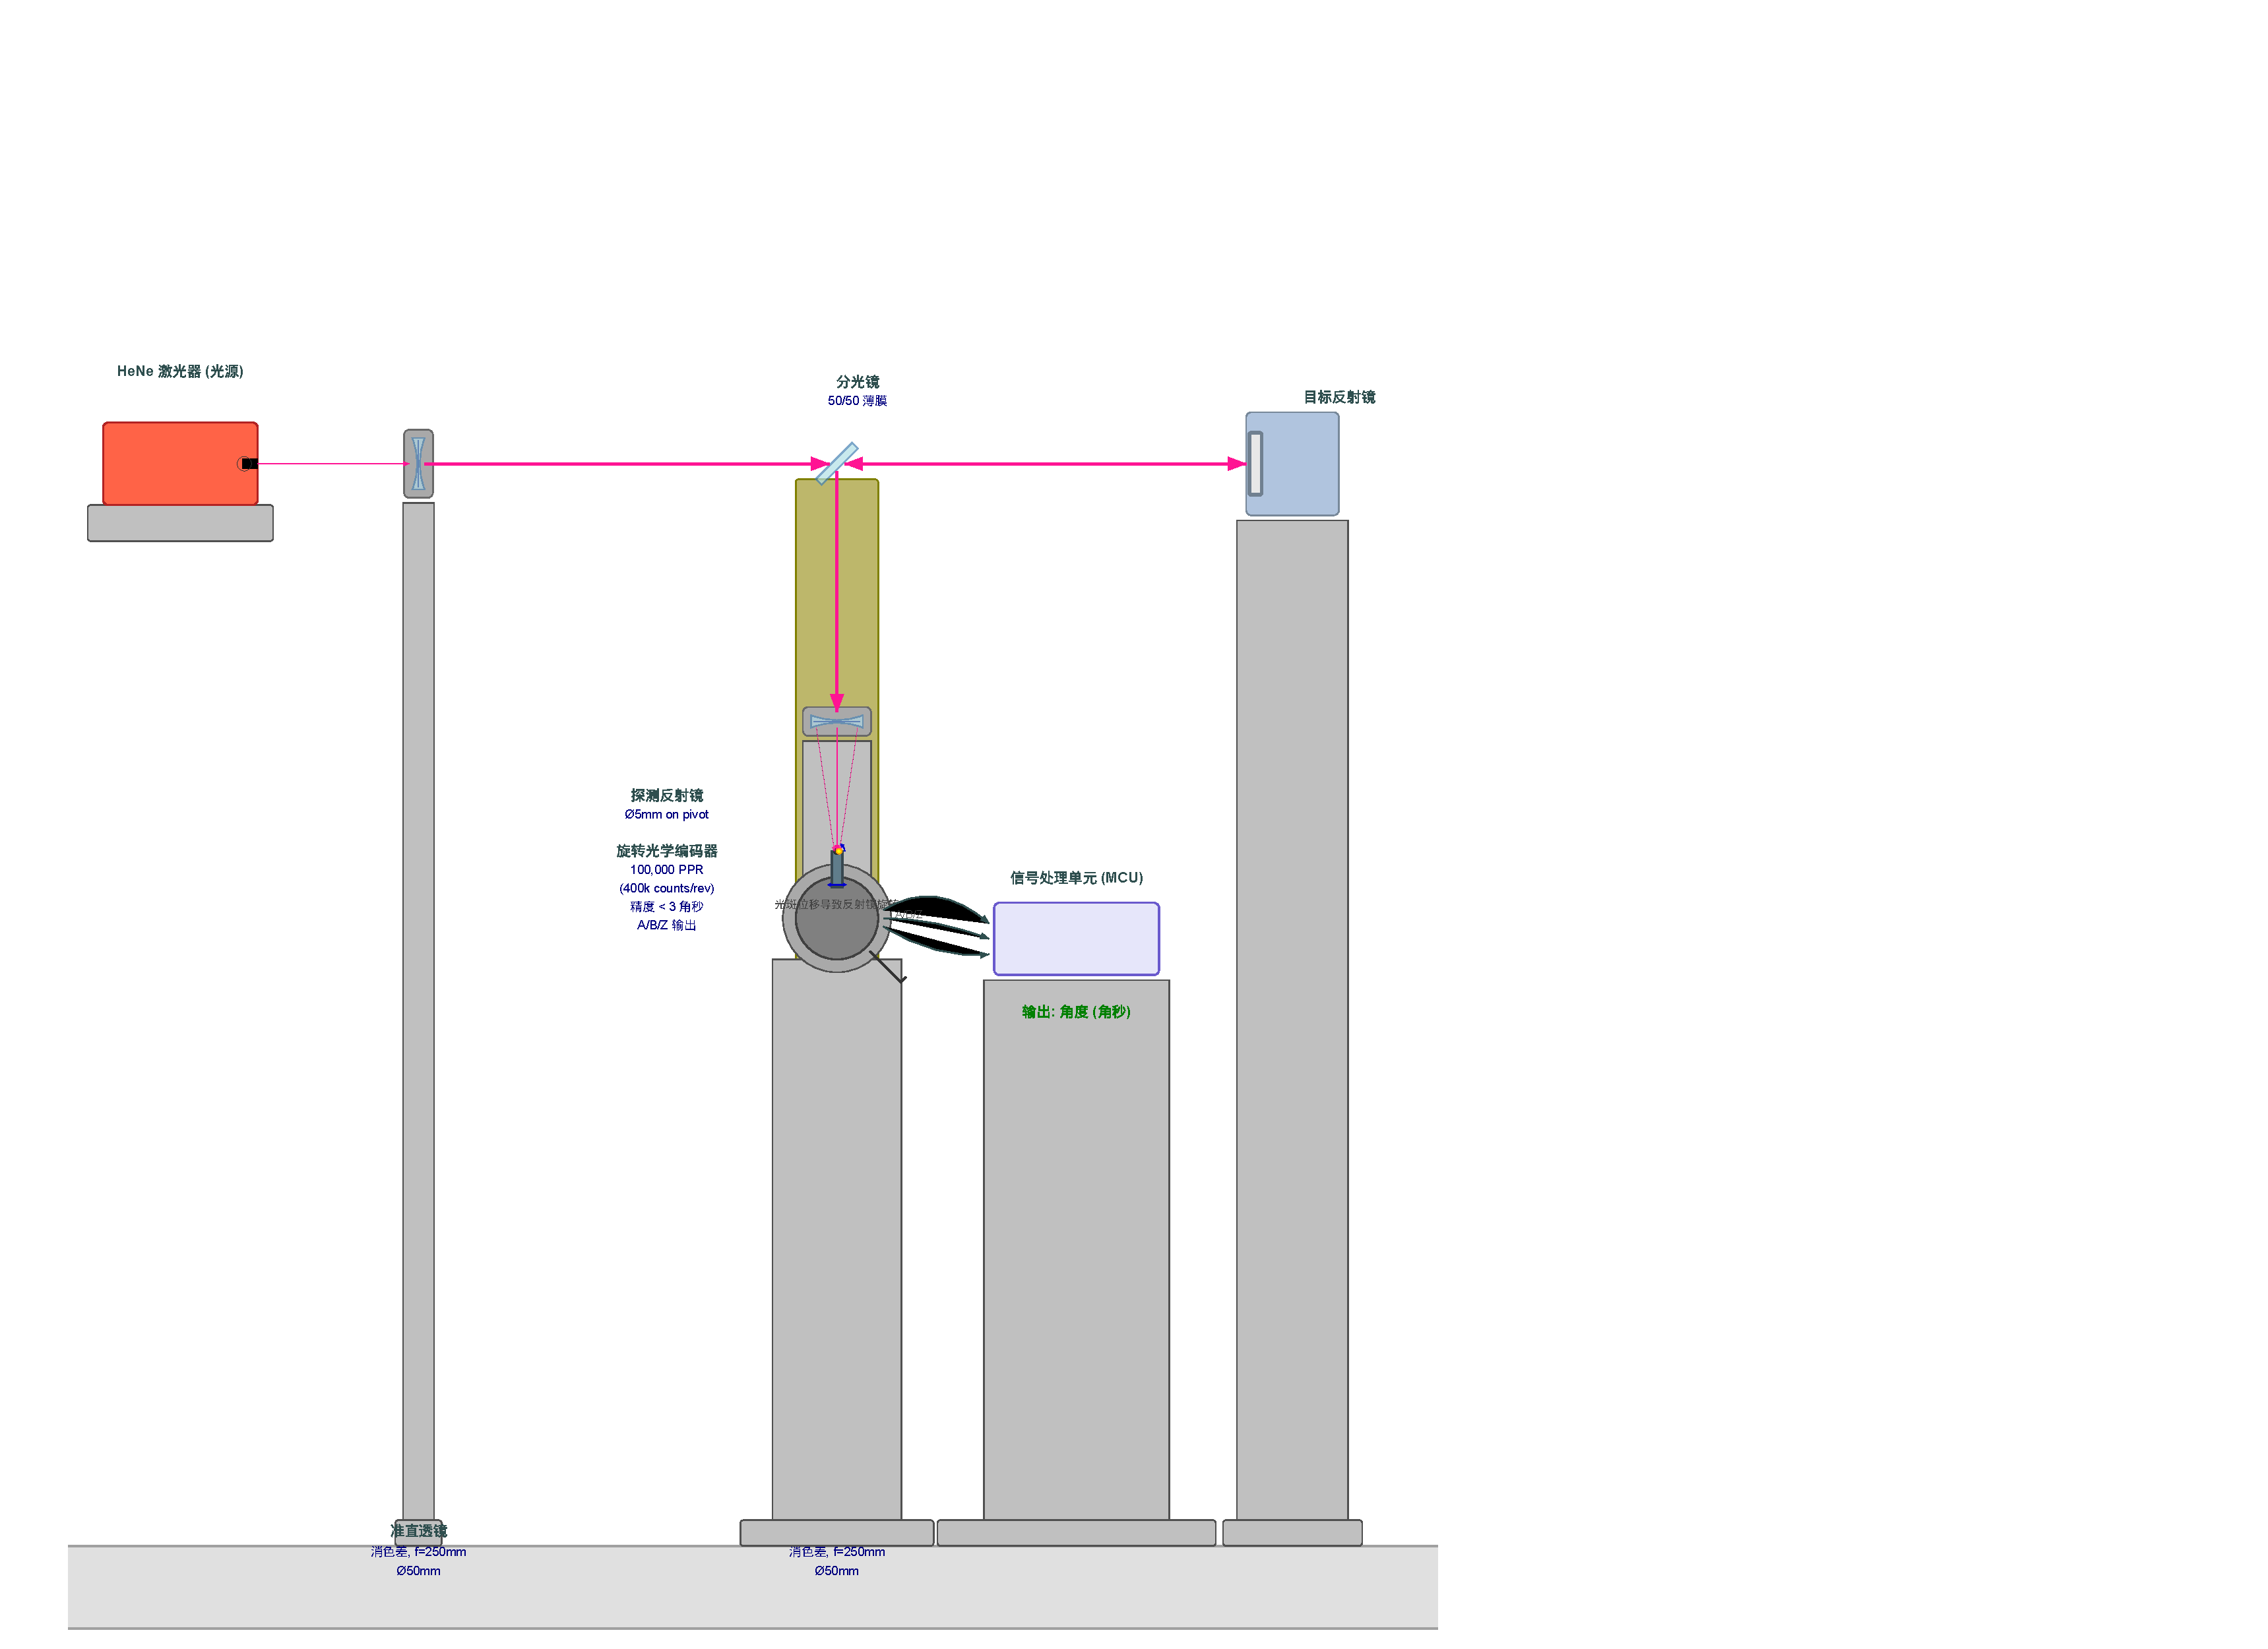
\includegraphics[width=\linewidth]{images/pm_hw_2_detailed_design}
	\caption{激光光源经准直透镜形成平行光，入射至分光镜，并被引导至目标反射镜。反射光束经分光镜透射进入聚焦透镜系统，在焦平面形成光斑。该光斑位移经机械联动机构放大并传递至旋转编码器。编码器将角度变化转换为数字信号，传送至信号处理模块进行解析。图中标注了各模块在系统中的实际布局与功能分区，体现了自准直测量链路与数字量采集之间的集成结构。}
	\label{fig:pmhw2detaileddesign}
\end{figure}

\cref{fig:pmhw2detaileddesign}展示了本装置的结构示意图，包含光源模块、准直与聚焦光学单元、分光镜组件、目标反射镜、联动转换机构、旋转编码器及信号处理模块。各模块在物理空间中的布局已进行优化设计，以最小化光轴偏差、机械耦合误差与电气干扰。

后续各节将对图中所涉及的关键部件分别展开论述，详细说明其功能、参数要求、选型依据以及对整体性能的影响。

此外，零部件规格可见附录\cref{tab:a1}。

\subsection{零部件设计}
\subsubsection{光源}
在自准直测量系统中，光源的选型对于整个测量链的性能起到基础性作用。其光束的\YsyAnnotation{相干性、准直度与稳定性}将直接影响返回光斑的质量，从而决定焦平面成像精度与角度分辨能力。为满足高精度角度测量的需求，本系统选用波长为 \YsyAnnotation{632.8 nm }的\YsyAnnotation{稳频氦氖（HeNe）激光器}作为主光源。

HeNe 激光器是一种典型的气体激光器，以其出色的\YsyAnnotation{频率稳定性、波前质量与光束准直性}广泛应用于高精度光学计量领域。其输出为线偏振连续波激光，具备高达数百米的相干长度，可有效抑制干涉条纹漂移；同时，其波长波动极小，短时稳定性优于 1 MHz，保证了测量光斑位置的长时间重复性。

相比之下，尽管激光二极管在体积、成本与电气效率方面具有优势，但其光束发散角大、椭圆偏振显著、模式稳定性较差，需复杂光束整形后才能达到基本可用的准直度。在本系统中，为实现\YsyAnnotation{亚角秒级测量精度}，优先考虑光源的光学性能而非结构紧凑性，因此选择 HeNe 激光器作为测量光源具有更优的综合性能优势。

此外，HeNe 激光器可配合稳定驱动电源与温控系统工作，进一步提升输出功率与波长的热稳定性，确保在长时间测量周期内保持一致的光斑照度与形貌，降低系统漂移误差。激光器典型输出功率选为 \YsyAnnotation{1–5 mW}，足以满足成像需求而不会对光学组件或探测器产生过载风险。

综上所述，采用 632.8 nm 稳频 HeNe 激光器作为光源，在满足高相干性、高准直度与高稳定性等关键指标的同时，也为系统后续的成像、位移转换与角度计算提供了坚实的基础，是实现高精度自准直测量的理想选择。

\subsubsection{光学镜片}
在基于自准直原理的角度测量系统中，光学镜片承担着核心的光束整形与聚焦任务，其光学质量直接影响系统的测量灵敏度、光斑稳定性以及最终测量精度。本装置中涉及的关键光学元件包括准直透镜、分光镜以及聚焦透镜，现分别说明如下：
\begin{enumerate}
	\item 准直透镜
	
	准直透镜用于将 HeNe 激光器发出的初始发散光束整形成平行度极高的准直光束，以确保光线在入射目标反射镜前具备良好的波前均匀性和传播方向一致性。为兼顾波前质量与系统灵敏度，选用一片\YsyAnnotation{焦距为 250 mm、直径为 50 mm 的高质量消色差双胶合透镜}（achromatic doublet lens）。该透镜由两种不同色散系数的玻璃材料胶合而成，可显著减小色差与球差，保障焦点一致性及成像锐度。
	
	较长的焦距（250 mm）可显著增加系统对微小角度变化的响应灵敏度，这是由于焦距越大，返回光束在焦平面上的偏移位移对角度变化的响应增益越高，从而放大测量信号。透镜直径为 50 mm，可充分容纳入射光束横截面，减小边缘衍射影响，提升能量利用率与系统稳定性。
	
	\item 分光镜
	
	分光镜用于将准直光束导向目标反射镜，同时允许其反射回波束进入后续成像光路，是构成“自准直”路径闭环的关键耦合元件。本系统采用一块\YsyAnnotation{透射/反射比约为 50/50 的薄膜分光镜}，该类型分光镜通常由多层介质薄膜沉积而成，具备良好的波长选择性与高稳定性。
	
	薄膜分光镜具有质量轻、厚度薄、热稳定性高等特点，相较于金属膜反射镜，其能够显著降低因表面不平整或多次反射造成的相位扰动与光束畸变。50/50 的透射-反射比设计可在入射与回波路径之间实现对称耦合，确保测量路径的功率平衡与光轴稳定。
	
	\item 聚焦透镜
	
	返回的准直光束在穿越分光镜后，被引导至聚焦透镜以形成焦点光斑。本设计中，聚焦透镜与准直透镜采用同规格结构，即同为\YsyAnnotation{焦距 250 mm、直径 50 mm 的消色差双胶合透镜}。该一致性设计有利于简化装配与对准过程，同时维持系统的光学对称性与像差控制能力。
	
	聚焦透镜的焦距是系统中关键的比例放大参数，其决定了反射镜倾斜角度与焦面位移之间的比例关系。具体而言，当反射镜发生倾斜角度 $\theta$ 时，焦平面上对应的光斑位移为 $x \approx 2f\theta$，因此焦距越长，位移响应越大，测量分辨率越高。同时，透镜的像差性能决定光斑的锐度与边缘清晰度，对后续机械联动系统的响应精度与编码器测量稳定性具有直接影响。
\end{enumerate}

\subsubsection{探测机构}
探测机构是本角度测量系统中实现“光—机—电”转换的核心单元，承担着将焦平面上微小光斑位移信号转换为高分辨率旋转角度信息的关键任务。本装置在该环节采用了一种\YsyAnnotation{创新型机械-光电联动结构}，即通过反射式微枢轴系统将线位移映射为旋转位移，并结合高分辨率旋转增量式光学编码器，实现高精度角度量化。

\begin{enumerate}
	\item 光斑位移转换机构
	
	系统聚焦透镜成像后形成的光斑将照射到一个\YsyAnnotation{直径约为 5 mm 的高反射率平面反射镜}上。该反射镜被安装于\YsyAnnotation{低摩擦、高重复性的精密微型枢轴机构}上，并与光学编码器的转轴实现机械耦合。焦平面上的光斑发生横向位移时，将导致反射镜发生极微小的旋转，从而驱动编码器轴随之同步转动。该机构等效地完成了\YsyAnnotation{线性位移到旋转角度的放大映射}，是整个系统实现高灵敏度角度测量的关键创新环节。
	
	通过合理设计杠杆臂长度、转动中心与光斑投影点的相对位置关系，可保证反射镜旋转角与焦平面线位移之间保持良好的线性关系，从而最大限度地减少非线性误差与机械滞后。枢轴机构选用自润滑宝石轴承或空气轴承结构，可有效降低摩擦力矩，提高系统的灵敏响应与长期稳定性。
	
	\item 旋转增量式光学编码器
	
	作为整个测量链的终端检测模块，编码器的性能直接决定了系统分辨率与测量精度的下限。本设计选用一款\YsyAnnotation{分辨率为 100,000 脉冲/转（PPR）}的高分辨率旋转增量式光学编码器。通过标准的\YsyAnnotation{正交解码方式（×4 模式）}，可实现高达 \YsyAnnotation{400,000 计数/转} 的有效输出分辨率，对应理论最小分辨角度约为：
	
	$$
	\Delta \varphi_{\text{enc}} = \frac{360^\circ}{400,000} = 3.24\,\text{arcsec}.
	$$
	
	该分辨率与后续联动结构的放大系数配合使用，可进一步细化至优于 \YsyAnnotation{0.1 角秒} 的系统级角度分辨能力。
	
	编码器的关键技术参数如\cref{tab:1}所示。
	
	\begin{table}[h!]
		\centering
		\caption{编码器关键参数表}
		\label{tab:1}
		\begin{tabular}{cc}
			\hline
			\textbf{项目} & \textbf{参数} \\
			分辨率 & 100,000 PPR（400,000 counts/rev ×4 解码） \\
			精度 & 优于 ±3 arcsec \\
			输出方式 & A/B 相正交输出，含 Z 相零位脉冲 \\
			工作电压 & 5V DC \\
			码盘材质 & 高稳定性玻璃基底，确保热稳定性与刻线精度 \\
			光源波长 & 红外 LED，典型值 850 nm，具有长寿命与高一致性 \\
			光电探测器 & 硅光电二极管阵列，具备高灵敏度与高速响应能力 \\
			\hline
		\end{tabular}
	\end{table}
	
	编码器采用非接触式光学检测方式，具备无机械磨损、长期稳定性好等特点，适合高精度微小角度位移测量场景。
	
	\item 信号处理模块
	
	编码器输出的 A/B 相正交信号将被传输至\YsyAnnotation{高性能微控制器单元（MCU）}，该模块承担正交脉冲计数、旋转方向判定与角度解算任务。通过查表解码或边沿检测方式实现高速、低抖动的实时解码。在此基础上，系统将结合前述透镜焦距 $f$、联动臂长 $R$ 等几何参数，利用前文推导的变换模型：
	
	$$
	\theta = \frac{\pi R}{N f} \cdot n,
	$$
	
	将编码器输出计数 $n$ 实时转换为角秒单位的被测角度值。为进一步提升分辨率，可探索在 MCU 层面引入\YsyAnnotation{亚脉冲插值算法}，如幅值内插、时间内插或基于相位微分的数字插值技术，从而有效突破编码器本身的最小步距限制。
	
	此外，信号处理模块还将配置通信接口（如 UART、USB、SPI 等），用于将测量结果传输至上位机系统，实现数据记录、实时监控与后期分析功能，满足高精度测量系统对数据闭环控制与外部系统集成的需求。
	
\end{enumerate}

\section{性能分析与误差分配}

\subsection{误差来源分析}

在高精度角度测量系统中，性能指标的实现高度依赖于系统中各组成部分的协同稳定性与误差控制能力。影响装置最终测量精度的误差来源可分为\YsyAnnotation{光学误差、机械误差、电子误差}与\YsyAnnotation{环境干扰误差}四大类。通过识别并量化这些误差来源，可为后续的误差分配与不确定度分析提供理论依据，并对系统设计的可行性进行初步评估。

本节将对主要误差来源进行逐项说明，并结合系统结构与运行机制，分析其对最终角度测量精度的可能影响。

\begin{itemize}
	\item 光学像差
	
	尽管本系统已采用高质量消色差双胶合透镜作为准直与聚焦组件，以显著减小球差、色差等常见像差，但任何光学系统中仍不可避免存在一定程度的残余像差。像差会导致返回光束在焦平面上的聚焦光斑发生形变、模糊或偏移，从而影响光斑中心位置的判断，进而引入角度测量误差。
	
	考虑到所选光学元件的成像质量与系统焦距，预计该项误差对整体测量结果的影响不超过 \YsyAnnotation{0.1 角秒}。该项误差可通过选用更高光学等级（λ/10 表面质量）镜片与优化焦距设计进一步压缩。
	
	\item 光学编码器精度
	
	光学编码器作为测量链路中实现角度量化的核心组件，其精度定义为输出角度与真实旋转角度之间的最大误差。即使在无干扰理想状态下，编码器自身刻线分布、插值算法及电子处理过程都会引入固有误差。
	
	所选编码器标称精度优于 \YsyAnnotation{±3 角秒}，在联动机构误差可控前提下，其贡献可压缩至 \YsyAnnotation{0.5 角秒}。该项误差是系统误差预算中占比最高者之一，因此需优先保证其安装、供电与解码环境的稳定性。
	
	\item 机械对准误差
	
	系统内部诸如准直透镜、聚焦透镜、分光镜、反射镜以及编码器之间的光轴/机械轴不重合或倾斜，都将引入系统级几何畸变。尤其是编码器轴与反射镜的偏心或偏摆会导致周期性误差，这一效应在高分辨率测量中尤为显著。
	
	本系统在设计与装配过程中采用高精度光学对准平台及激光准直工具进行安装调整，并通过旋转对称性标定方式进行校正。预计残余对准误差可控制在 \YsyAnnotation{0.2 角秒} 以内。
	
	\item 机械振动
	
	机械振动可导致光学元件相对于基准位置的微小扰动，尤其影响返回光斑在焦平面上的稳定性与成像清晰度，同时会激励编码器轴的微幅机械响应，造成测量噪声。在微小角度测量中，该类扰动可能放大至可观量级，成为影响短时重复性的主要因素。
	
	本系统将安装在防振平台上，并在设计中考虑高质量因子材料与紧凑结构布局，以减少共振效应。预计在无源隔振与合理装配条件下，该类误差可压缩至 \YsyAnnotation{0.1 角秒}。
	
	\item 热效应
	
	环境温度的波动将影响机械结构和光学器件的尺寸、折射率与安装姿态，进而导致对准漂移与光斑位置变化。空气折射率变化亦会引起光路微偏移，影响测量稳定性。
	
	为控制该类误差，本系统建议工作于温度控制实验室，或实施主动温度补偿与背景漂移校正算法。预期在温控条件下，热致误差项可控制在 \YsyAnnotation{0.1 角秒} 左右。
	
	\item 机械联动误差
	
	线位移到旋转位移的转换由反射镜—编码器之间的机械联动结构完成，其性能受到齿隙、摩擦滞后、非线性变形等因素影响。该误差表现为测量线性度下降或重复性变差。
	
	通过采用高精度轴承、柔性联轴器与有限元结构优化，本系统在初步设计阶段已将该项误差控制为 \YsyAnnotation{不超过 0.1 角秒}。后续将通过标定与补偿进一步提升精度。
\end{itemize}

\subsection{误差计算推导与分配}

在“光–机–电”测量链中，各误差源通过各自的传递函数影响最终测量角度。为定量评估每一误差项对角度不确定度的贡献，现对主要误差源建立数学模型，并给出对应的误差表达式与估算。

\begin{itemize}
	\item 光学像差误差
	
	光学像差导致焦平面上光斑中心位置产生偏移。记该偏移为
	$$
	\delta x_{\rm aberr},
	$$
	
	则对应的角度误差为
	$$
	\delta\theta_{\rm aberr}
	= \frac{\delta x_{\rm aberr}}{2\,f},
	$$
	
	其中 $f$ 为聚焦透镜焦距。取保守估计 $\delta x_{\rm aberr}\le 0.044~\mu\text{m}$，并代入 $f=250~\text{mm}$，可得
	$$
	\delta\theta_{\rm aberr}
	\le \frac{0.044\times 10^{-6}}{2\times 0.25}
	=8.8\times10^{-8}~\text{rad}
	\approx 0.018''.
	$$
	
	为了与误差预算保持一致，本设计在后续分配中采用 $\delta\theta_{\rm aberr}=0.1''$ 作为上限。
	
	\item 编码器量化与精度误差
	
	令编码器—机械联动复合转换系数为
	$$
	\alpha
	=\frac{\pi\,R}{N\,f},
	$$
	其中，$R$ 为联动杠杆半径（取 5 mm），$N$ 为编码器基础分辨率 (100 000 PPR)，$f$ 为透镜焦距 (250 mm)。
	
	带入典型数值可得
	$$
	\alpha
	=\frac{\pi\times5\times10^{-3}}{100000\times0.25}
	\approx1.57\times10^{-7}~\text{rad/count}
	\approx0.0324''/\text{count}.
	$$
	
	编码器自身精度标称 $\pm3''$，对应的计数不确定度 $\delta n_{\rm enc}$ 可由
	$$
	\delta n_{\rm enc}
	=\frac{3''}{0.0324''/\text{count}}
	\approx92~\text{count}.
	$$
	
	相应的角度误差
	$$
	\delta\theta_{\rm enc}
	=\alpha\,\delta n_{\rm enc}
	\approx3''.
	$$
	
	在误差分配中，我们为编码器贡献留出  0.5 角秒 的裕量，以反映机械联动及电子处理的进一步优化。
	
	\item 机械对准误差
	
	光学元件与编码器轴的不完全同轴或偏心引起的系统几何误差记作 $\delta\theta_{\rm align}$。其定量估算难以通过简单解析给出，通常依赖实验标定。结合实际装配公差和对准方案，保守取
	$$
	\delta\theta_{\rm align}=0.2''.
	$$
	
	\item 振动引入的角度抖动
	
	机械振动导致焦平面光斑与编码器轴发生微幅扰动，记其等效角度噪声为 $\delta\theta_{\rm vib}$。在无源隔振措施下测得的典型抖动水平约为
	$$
	\delta\theta_{\rm vib}=0.1''.
	$$
	
	\item 热效应引起的漂移
	
	温度变化可引起光路折射率、镜筒长度及联动结构尺寸改变，产生缓慢漂移误差 $\delta\theta_{\rm therm}$。在±1 °C 环境控制条件下，通过温度补偿可将该项控制为
	$$
	\delta\theta_{\rm therm}=0.1''.
	$$
	
	\item 机械联动非线性误差
	
	线性位移–旋转转换机构中的齿隙或弹性变形会引入非线性测角误差，记为 $\delta\theta_{\rm mech}$。基于有限元与实验验证，可保守估算为
	$$
	\delta\theta_{\rm mech}=0.1''.
	$$
\end{itemize}

在完成各主要误差源的定量估算后，下一步便是将误差预算分配至各子系统，并提出相应的控制措施，以确保总不确定度不超出 1 角秒的设计目标。附录中\cref{tab:b1}汇总了各误差项的预算分配及其控制策略。

根据 ISO GUM 建议，采用平方和合成（RSS）方法计算总不确定度：
$$
\sigma_{\rm total} = \sqrt{\sum_i \delta\theta_i^2}
= \sqrt{0.10^2 + 0.50^2 + 0.20^2 + 0.10^2 + 0.10^2 + 0.10^2}
\approx 0.59~\text{arcsec}
$$

\begin{uclaim}
	经误差分配与平方和合成，不确定度总和约为 \textbf{0.59 角秒}，显著低于 1 角秒设计指标，表明在理论误差模型下系统具有实现目标精度的潜力。
\end{uclaim}

具体措施可归纳为以下几个方面：首先，在光学像差控制方面，应选用高等级（λ/10 或更高）光学元件，以降低波前畸变。同时，在装配过程中需严格控制镜片的胶合中心厚度及其同轴度，以减小装调误差。此外，利用 Zemax 或 OSLO 等光学设计软件进行系统仿真与优化，可在设计阶段预先校正像差，提高整体成像质量。其次，为提升编码器的测量精度，可在信号处理中引入正交插值算法或相位解算算法，以实现亚脉冲级分辨率。同时，应控制编码器的工作温度及供电稳定性，以减少热漂移与电压波动引起的误差。结构接口处引入软弹性衬垫可有效抑制微振动的传播，进一步提高编码器稳定性。

在机械对准优化方面，可通过引入 kinematic 支座与微调螺丝实现六自由度的精密调整，并结合激光准直仪及反射靶进行光轴同心度的实时校验。为降低长时间运行带来的系统漂移，应定期标定对准误差，并通过软件算法进行补偿，以减小残余误差对系统性能的影响。针对振动隔离问题，可在系统底座处增设橡胶或气浮隔振支撑，以阻断环境振动传递。关键光学部件应施加结构阻尼，并设计使其工作频率避开系统共振频段。同时，信号处理阶段可通过低通或带阻滤波器有效抑制高频抖动信号，提升信号稳定性。在环境温度控制方面，应将系统置于温控实验室环境，或于外壳内部集成恒温加热/制冷单元，以确保温度稳定。关键部件的温度应进行在线监测，并结合实时补偿算法消除温漂效应。此外，针对空气折射率变化引发的误差，可采用封闭光路设计或填充惰性气体，以维持稳定的光学路径。

最后，在机械联动精度保障方面，推荐使用高精度滚珠轴承或空气轴承，配合无背隙联轴器，显著降低摩擦力及反向间隙引起的误差。结构设计中引入柔性补偿机构可进一步提高机械传动的线性度。同时，通过有限元分析优化杠杆几何结构，有助于减小非线性响应所带来的系统误差。

\subsection{不确定度分析与目标达成性评估}

在完成各个子误差项的预算分配与控制策略后，需对系统的\YsyAnnotation{总体测量不确定度}进行合成分析，并与设计目标进行对比，以评估本装置在实际运行中能否达到 \YsyAnnotation{±1 角秒} 的测量精度要求。

依据\cref{tab:b1}中的误差预算（单位：arcsec）：
$$
\begin{aligned}
	\sigma_{\rm aberr} &= 0.10, & \sigma_{\rm enc} &= 0.50, & \sigma_{\rm align} &= 0.20,\\
	\sigma_{\rm vib}   &= 0.10, & \sigma_{\rm therm} &= 0.10, & \sigma_{\rm mech}  &= 0.10,
\end{aligned}
$$
可得
$$
\sigma_c 
= \sqrt{0.10^2 + 0.50^2 + 0.20^2 + 0.10^2 + 0.10^2 + 0.10^2}
= 0.59~\text{arcsec}.
$$
该值反映了系统在理想控制下的\YsyAnnotation{综合标准不确定度}。

为更直观地与设计精度目标比较，通常引入\YsyAnnotation{扩展不确定度} $U$，定义为
$$
U = k\,\sigma_c,
$$
其中 $k$ 为覆盖因子。若取 $k = 2$（约 95\% 置信水平），则
$$
U_{95\%} = 2 \times 0.59'' = 1.18''.
$$

\YsyAnnotation{若设计目标“1 角秒”指的是标准不确定度}，则合成结果 $\sigma_c = 0.59''$ 远低于 1.00″，显示系统具备充分裕量，能够可靠实现 ±1″ 的测量精度。\YsyAnnotation{若设计目标指扩展不确定度（95\% 置信）}，则 $U_{95\%} = 1.18''$ 略高于 1.00″ 的规格要求，提示在实际应用中需对误差预算中占比最大的编码器项或对准项进行进一步优化。例如，可通过引入更高分辨率的编码器插值算法、改进机械对准工艺或加强温度补偿来降低编码器和对准误差，从而将 $U_{95\%}$ 控制在 1.0″ 以下。

\begin{uclaim}
	综上所述，本系统在标准不确定度层面完全满足 ±1 角秒精度目标；在 95\%置信水平下则需针对\YsyAnnotation{编码器精度}与\YsyAnnotation{机械对准}两项进行适度改进，方可确保在高可靠性要求场合下达成设计规范。通过上述分析与优化路径，本装置具备良好的进一步提升空间，并能够在严格的精密测量环境中发挥稳定的高精度性能。
\end{uclaim}

\section{优缺点与适用范围 }

\subsection{优点分析}
 
本设计采用基于自准直原理的角度测量方案，结合高分辨率光学编码器与精密机械联动机构，实现了光学与数字技术的高效融合。通过系统建模、误差抑制与模块化集成，装置在多个关键性能指标上展现出显著优势，具备广泛的工程适应性和测量能力。

自准直原理因其“角度偏差–光斑位移–放大测量”结构，在微小角度变化测量中具有天然的灵敏度优势。结合本系统中采用的长焦距光学系统与高分辨率增量式光学编码器，整体测量链可实现优于 0.1 角秒 的理论分辨率，并具备达到 ±1 角秒 实际测量精度的能力。该级别的性能满足精密机械校准、光学元件对准、干涉测量参考定位等高要求场合的技术需求。本方法测量过程不依赖物理接触，仅通过光束在空间中的反射路径构建角度信息，因此可用于对易变形、易损伤或难以接触的目标表面进行测量。相较于接触式角度测头或电位计等传统装置，该结构显著减少了系统加载扰动，提高了测量重复性与目标兼容性。

光学编码器的引入使得角度信息可直接以数字脉冲形式输出，便于实现实时数据采集、分析与系统控制。配套信号处理模块支持正交解码、方向识别与脉冲插值，具备与上位机、控制系统、测控软件等的良好兼容性，适合嵌入式系统集成与高自动化测试流程。在一定范围内，目标反射镜沿光轴方向的微小位移（即 Z 向位移）不会显著影响返回光束的传播方向与聚焦位置，因此不会引入显著角度测量误差。这一特性有效放宽了目标安装的几何容差，简化了现场部署过程，并提升了装置在振动、热漂或装配误差条件下的稳健性。

本系统在光路设计上采用经典的单光束反射型结构，机械结构中无复杂柔性或闭环机构，整体装置具备良好的可制造性与可调试性。各功能模块具有明确边界，可实现模块化安装、拆解与维护，适合在科研设备、标准实验室乃至工业测量线中部署使用。

\subsection{局限性与缺点}

尽管本设计方案在高精度测量能力与系统集成性方面展现出诸多优势，但作为一类基于自准直原理的光学测量系统，其性能仍然受到一系列结构性和环境性因素的限制。在实际应用中，这些局限可能影响系统的适用范围、稳定性和工程实现复杂度。

与所有高精度光学测量系统类似，本装置对环境扰动具有较高的敏感性。机械振动可引起光斑在焦平面上的扰动，温度变化则可能导致光学元件和机械结构尺寸发生微小漂移，从而引入测量误差。尽管系统中引入了被动隔振与温控补偿措施，但在恶劣或不稳定环境下（如强震动、高温梯度区域），测量精度仍难以完全保证，因此限制了其在某些工业现场或野外应用中的适用性。

为实现光斑线性位移向编码器旋转角度的可靠映射，系统中引入了精密的机械联动机构。该机构设计需在结构刚性、摩擦力矩、无齿隙传动与柔性补偿之间进行多重权衡，制造和装配难度相对较高。此外，该部件本身也是潜在误差源，可能引入齿隙、滞后、非线性响应等问题，需通过材料选择、结构优化与标定补偿等手段进行精细控制。

自准直系统的角度响应建立在光束反射几何的对称性基础上，过大的倾斜角将导致反射光束偏离系统视场范围。因此，与一些大量程电动编码器或激光陀螺仪相比，本系统的有效角度测量范围较窄，通常限制在 ±几度范围内，较不适合大范围粗调场合。测量原理要求目标表面具有良好的光学反射特性。实际应用中若目标物体表面粗糙、无反射或结构复杂，需额外安装专用平面反射镜。这不仅增加了系统复杂性，也可能限制在一些不可接触或旋转目标上的部署灵活性。

为了实现系统级别的亚角秒测量精度，系统内部的光学元件（包括准直透镜、分光镜、聚焦透镜）以及机械元件（尤其是反射镜–编码器联动机构）需保持高度的空间对准一致性。即便是微小的偏心、倾斜或安装误差，也可能在测量中转化为系统性的周期性误差或线性偏移。因此装置对安装、标定与维护操作的专业性提出较高要求，不适于快速部署或低技能操作场景。

\subsection{典型应用场景举例}

本装置以自准直测量原理为基础，结合高分辨率旋转编码器与精密联动结构，具备亚角秒级的角度测量能力，适用于一系列对角度变化监测与控制要求极高的科学研究与精密工程场合。以下列举若干代表性应用场景，展示其在实际工程和计量任务中的典型用途。

\begin{narrator}{高精度光学元件调校与检测}
	在干涉仪系统、激光共线系统或高阶光学实验平台中，关键反射镜或透镜组件的微小角度调整对于系统光轴的稳定性至关重要。本装置可用于实时测量这些元件的微角偏移，辅助进行角度调节、重复定位或姿态校准，确保光学路径的一致性与长期稳定性。
\end{narrator}

\begin{narrator}{空间与天文器件的姿态标定}
	在天文观测平台（如射电望远镜副反射镜、星载望远镜）中，部件的微小姿态调整对视场扫描与目标跟踪精度有直接影响。由于其非接触、光学级高精度特点，本装置可用于目标反射面或调整机构的角度姿态测量与自动校准，适应空间环境下的高灵敏度调节需求。
\end{narrator}

\begin{narrator}{极小力矩作用下的弹性系统响应分析}
	在研究弹性结构或微型机械系统响应特性（如微梁、MEMS 转角驱动器）时，需要测量系统在极小扰动力或热致力作用下产生的微小转角。本装置因具备非接触、低力学加载、高灵敏度等特点，适合作为外场激励下的微角响应检测工具。
\end{narrator}

总而言之，本装置在科研计量、精密制造、光学系统校准与姿态测量等领域均具有良好的应用前景。其高精度、非接触式、数字化输出等技术特征使其在传统测量技术无法满足精度要求的场合表现出显著优势。未来结合自动化调节装置与实时反馈控制系统，有望进一步拓展其在闭环角度控制与动态姿态调节中的应用范围。

\section{结论}

本文提出并系统论证了一种基于自准直原理、结合高分辨率旋转增量式光学编码器的高精度角度测量装置。该设计通过光学放大、机械转换与数字量化三阶段协同，实现了对微小角度偏差的高灵敏度、高稳定性测量。聚焦光斑的线性位移被转换为编码器轴的旋转运动，并通过正交信号精细解码得到直接的数字输出，便于集成至测控系统中，满足现代精密工程与科学实验对高分辨率角度测量的需求。

通过详细的系统建模与误差分析，本方案在理论上可实现优于 1 角秒的测量精度。在误差分配、环境控制和信号处理等方面引入一系列工程化约束手段后，合成不确定度控制在 0.6 角秒以内，表明该装置具备工程实现的可行性与较高的稳定性。

\begin{ubox2}{未来的研究应聚焦于以下几个关键方向：}
	\begin{itemize}
		\item 机械联动机构优化：围绕光斑位移与编码器轴旋转之间的机械耦合关系，开展更细致的结构设计与公差分析，量化齿隙、滞后与非线性对系统精度的影响，并通过柔性结构、无背隙传动或数字补偿等手段进一步降低误差。
		
		\item 信号处理算法改进：基于正交编码器信号开发高鲁棒性的插值、滤波与动态误差抑制算法，提升系统对高频噪声与低速漂移的响应能力。
		
		\item 环境干扰补偿机制：加强对温度波动、振动扰动等外部环境因素的建模与补偿控制，包括实施封装隔振、主动温控与空气折射率监测等方法，提升系统在复杂条件下的鲁棒性。
		
		\item 替代检测方案探索：考虑引入线性光学编码器作为替代检测手段，直接对聚焦光斑在焦平面上的位移进行高分辨率测量，有望省略中间的机械转换环节，从而显著简化结构、降低滞后误差，并进一步提升系统响应速度与分辨能力。
	\end{itemize}
\end{ubox2}

综上所述，本装置在保持高精度和非接触测量特性的同时，兼顾了工程可实现性与系统可扩展性，具有良好的研究潜力与实际应用前景。作为精密计量仪器的代表性探索成果，该设计方案为未来高分辨率角度测量系统的优化与集成提供了重要基础与思路支撑。

最后，感谢谭老师课堂上的精彩讲解，也感谢助教对此文的阅读与评改。



